
\documentclass{standalone}
\usepackage[svgnames]{xcolor}
\usepackage{pgfplots}
\pgfplotsset{compat=newest}
\usepackage[sfdefault]{FiraSans}
\usepackage{FiraMono}
\renewcommand*\familydefault{\sfdefault}
\begin{document}
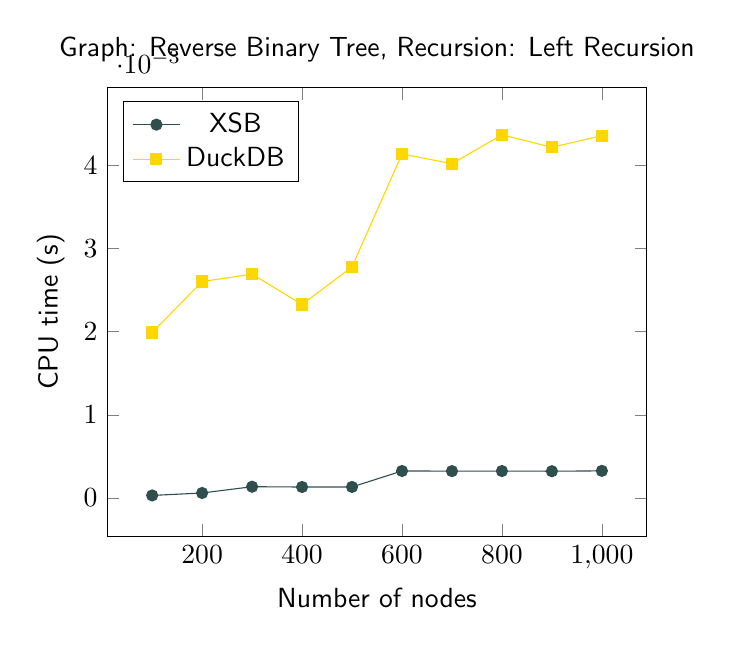
\begin{tikzpicture}
    \begin{axis}[
        title={Graph: Reverse Binary Tree, Recursion: Left Recursion},
        xlabel={Number of nodes},
        ylabel={CPU time (s)},
        legend pos={north west},
        ymax=0.004931799999999986
    ]
    \addplot+[DarkSlateGray, mark options={color=DarkSlateGray}] coordinates {(100,3.0799999999999576e-05) (200,6.019999999999984e-05) (300,0.0001356000000000002) (400,0.00013219999999999958) (500,0.0001327999999999994) (600,0.0003247999999999996) (700,0.0003233999999999996) (800,0.00032399999999999974) (900,0.0003219999999999998) (1000,0.00032619999999999996)};
\addlegendentry{XSB}
\addplot+[Gold, mark options={color=Gold}] coordinates {(100,0.0019905999999999978) (200,0.0026026000000000217) (300,0.002692199999999978) (400,0.002326399999999995) (500,0.002779200000000004) (600,0.004137799999999992) (700,0.004020199999999985) (800,0.0043669999999999985) (900,0.004217199999999999) (1000,0.0043574)};
\addlegendentry{DuckDB}

    \end{axis}
\end{tikzpicture}
\end{document}
